\section{Экспериментальное исследование}
Предложенный механизм диагностики ошибок был реализован на платформе .NET как часть проекта YaccConstructor; основным языком разработки являлся F\#~\cite{FSharp}. Данная реализация является модификацией ранее реализованного в рамках проекта алгоритма ослабленного синтаксического анализа регулярной аппроксимации динамически формируемого выражения.

Модифицированный алгоритм был протестирован на серии тестов с целью проверки работоспособности. Данные тесты проверяли, что алгоритм строит корректные множества $errors$ и $probErros$ ребер входного графа. Для каждого теста специфицировалась грамматика на языке YARD и в явном виде задавался граф конечного автомата, ребра которого были промаркированы лексемами входной грамматики. Входные графы для данных тестов содержали как ветвления, так и циклы. На всех тестах модифицированный алгоритм корректно строил множества $errors$ и $probErros$. Кроме того, на всех тестах, входные графы которых не содержали циклов, модифицированный алгоритм точно определял все ошибочные ребра входного графа, то есть $probErros$, в данном случае, являлось пустым множеством.

Также на нескольких сериях синтетических тестов была протестирована производительность модифицированного алгоритма. Анализ промышленного проекта по миграции базы данных с MS-SQL Server 2005 на Oracle 11gR2 показал, что запросы часто формируются конкатенацией фрагментов, каждый из которых формируется с помощью ветвлений или циклов. Ниже приведена входная грамматика, использованная в данных тестах.
$$
\begin{array}{crcl}
& start\_rule &::=& s \\
& s & ::= & s \mbox{\texttt{ PLUS }} \mbox{\texttt{n}}\\
& n & ::= & \mbox{\texttt{ONE | }} \mbox{\texttt{TWO | }} \mbox{\texttt{THREE | }} \mbox{\texttt{FOUR | }} \mbox{\texttt{FIVE | }} \mbox{\texttt{SIX | }} \mbox{\texttt{SEVEN}}
\end{array}
$$
Входные графы представляли собой конкатенацию базовых блоков без циклов. Каждая серия тестов характеризовалась тремя параметрами: 
\begin{itemize}
  \item $height$~--- количество ветвлений в базовом блоке;
  \item $length$~--- максимальное количество повторений базовых блоков;
  \item $errorBranches$~--- количество веток в базовом блоке, содержащих ошибочное ребро (на рис.~\ref{block} изображен базовый блок без ошибочных ребер, а на рис.~\ref{errorBlock} --- базовый блок с двумя выделенными ошибочными ребрами).
\end{itemize}

\begin{figure}[h!]
 \centering
 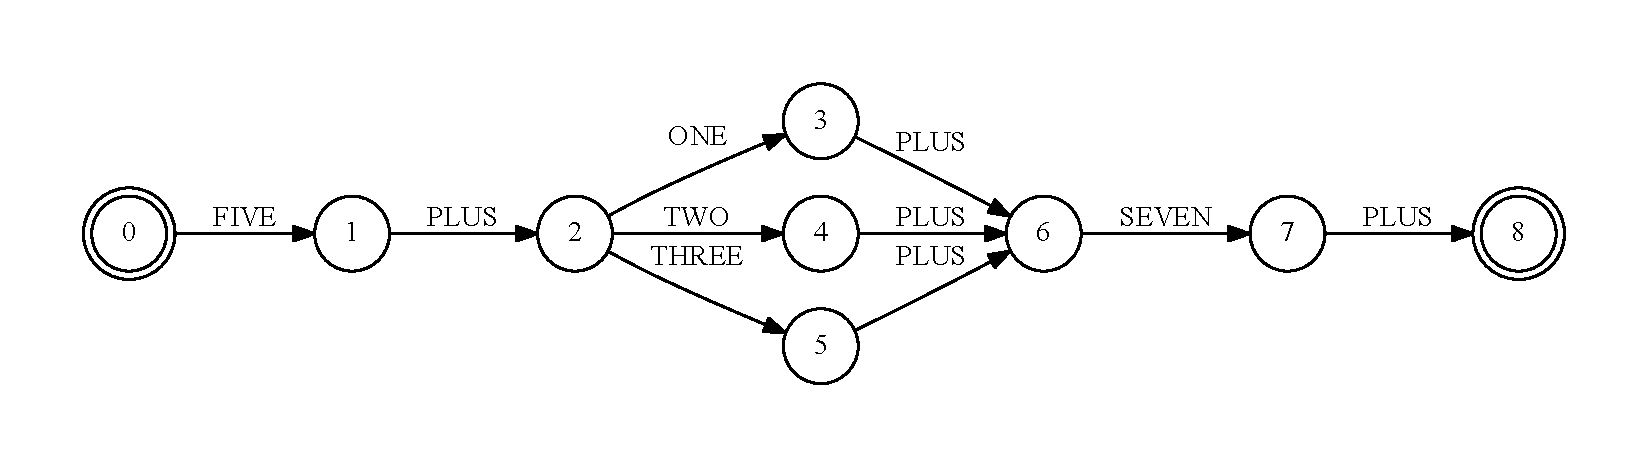
\includegraphics[width=15cm]{pictures/block_black.pdf}
 \caption{Базовый блок при $height=3, errorBranches=0$}
 \label{block}
\end{figure}

\begin{figure}[h!]
 \centering
 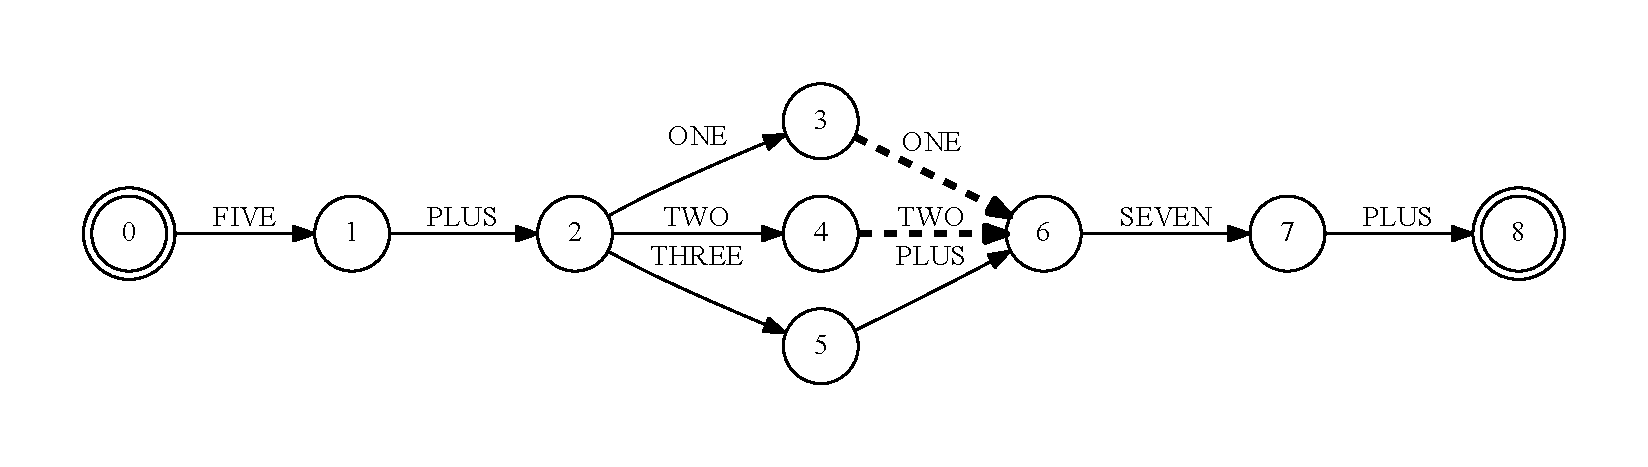
\includegraphics[width=15cm]{pictures/errorBlock_black.pdf}
 \caption{Базовый блок при $height=3, errorBranches=2$}
 \label{errorBlock}
\end{figure}

Замеры времени работы алгоритмов проводились на машине со следующими техническими характеристиками: Intel(R) Core(TM) i7-3630QM CPU @ 2.40GHz, RAM: 8.0~GB, процессор x64.

Каждая серия объединяет набор из 50 тестов, каждый из которых содержит одинаковое количество ветвлений в базовом блоке, при этом количество повторений блока совпадает с порядковым номером теста ($length = i$, для теста с номером $i$). Для каждого теста измерялось время, затраченное на синтаксический анализ. Измерения проводились 10 раз, после чего усреднялись. График, представленный на рис.~\ref{compare}, иллюстрирует сравнение времени работы алгоритма синтаксического анализа до и после модификаций. Можно заметить, что выполненная модификация существенно увеличивает продолжительность анализа. Причина этого в том, что выполненная модификация является прототипом, а в будущем планируется улучшить производительность путем улучшения реализации. График на рис.~\ref{withErrors} демонстрирует зависимость времени работы модифицированного алгоритма от количества повторений базового блока и количества веток, содержащих ошибочное ребро, в каждом из них. Наблюдается уменьшение времени работы модифицированного алгоритма при увеличении количества ошибочных ребер. Одной из причин этого является уменьшение количества корректных префиксов внутреннего графа при увеличении количества ошибочных ребер.

\begin{figure}[h!]
 \centering
 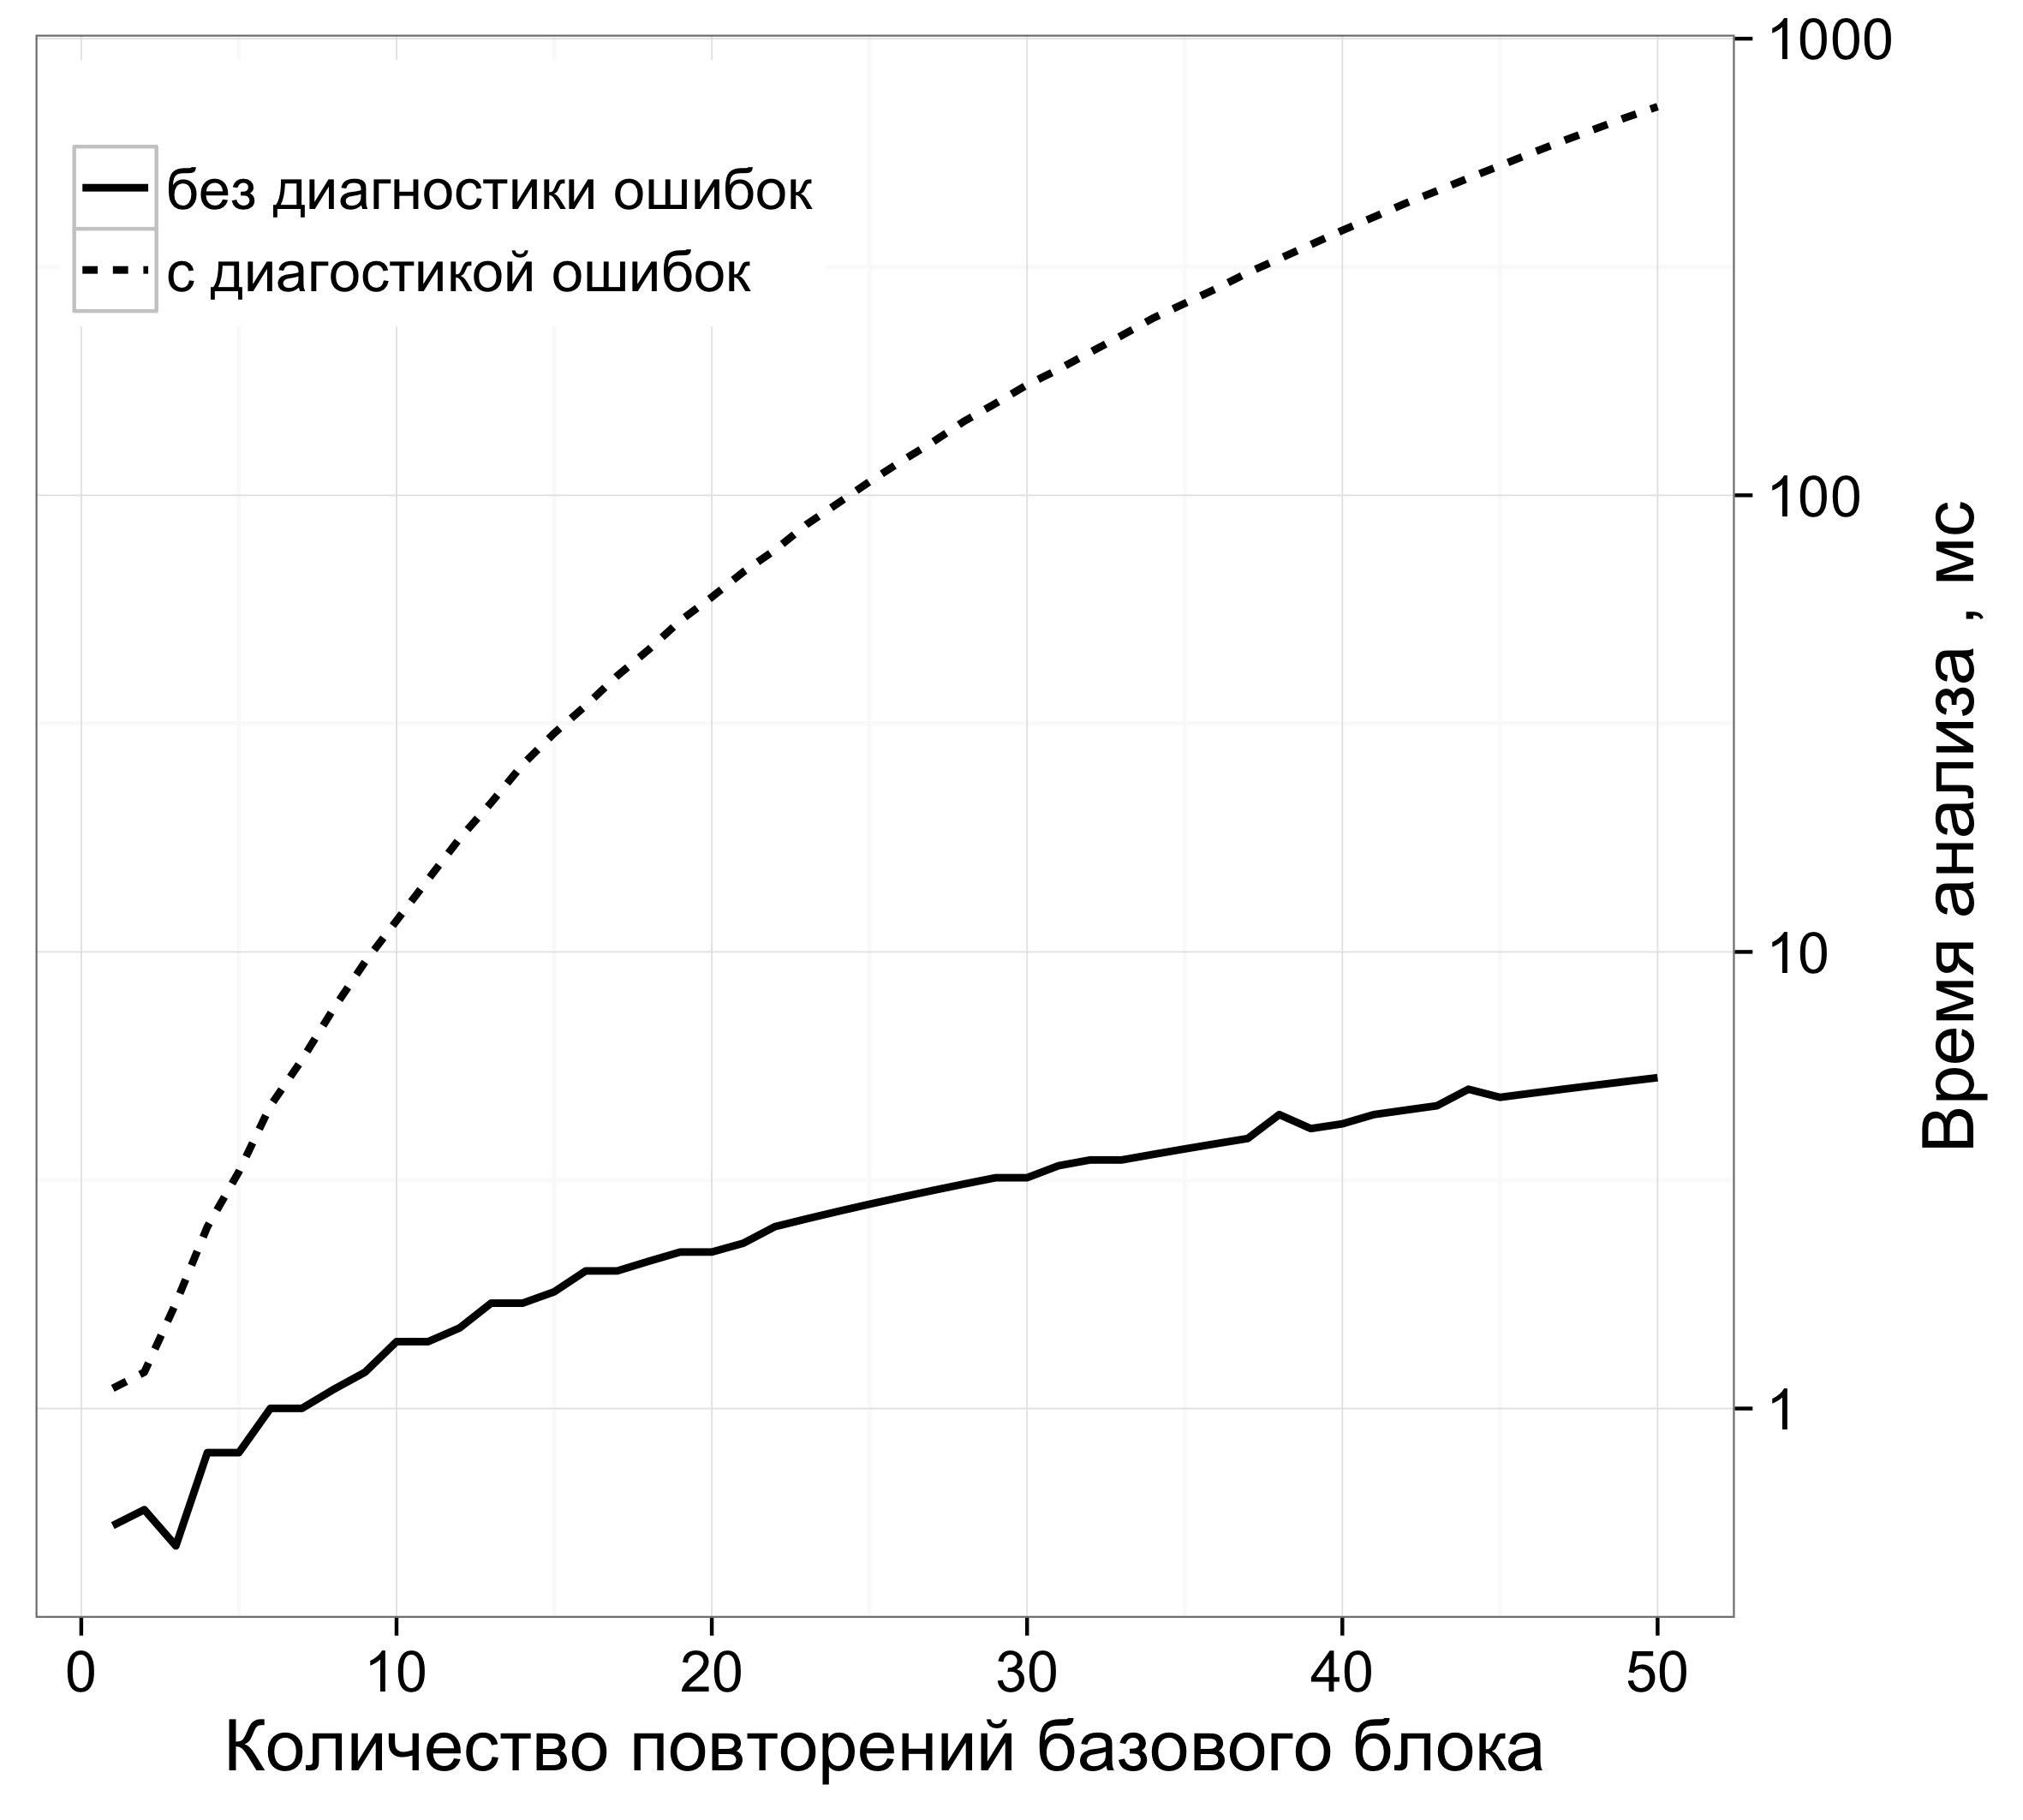
\includegraphics[width=11cm]{pictures/compare_black.png}
 \caption{Сравнение времени работы алгоритма синтаксического анализа до и после модификаций, при $height=4, errors=0$}
 \label{compare}
\end{figure}
\begin{figure}[h!]
 \centering
 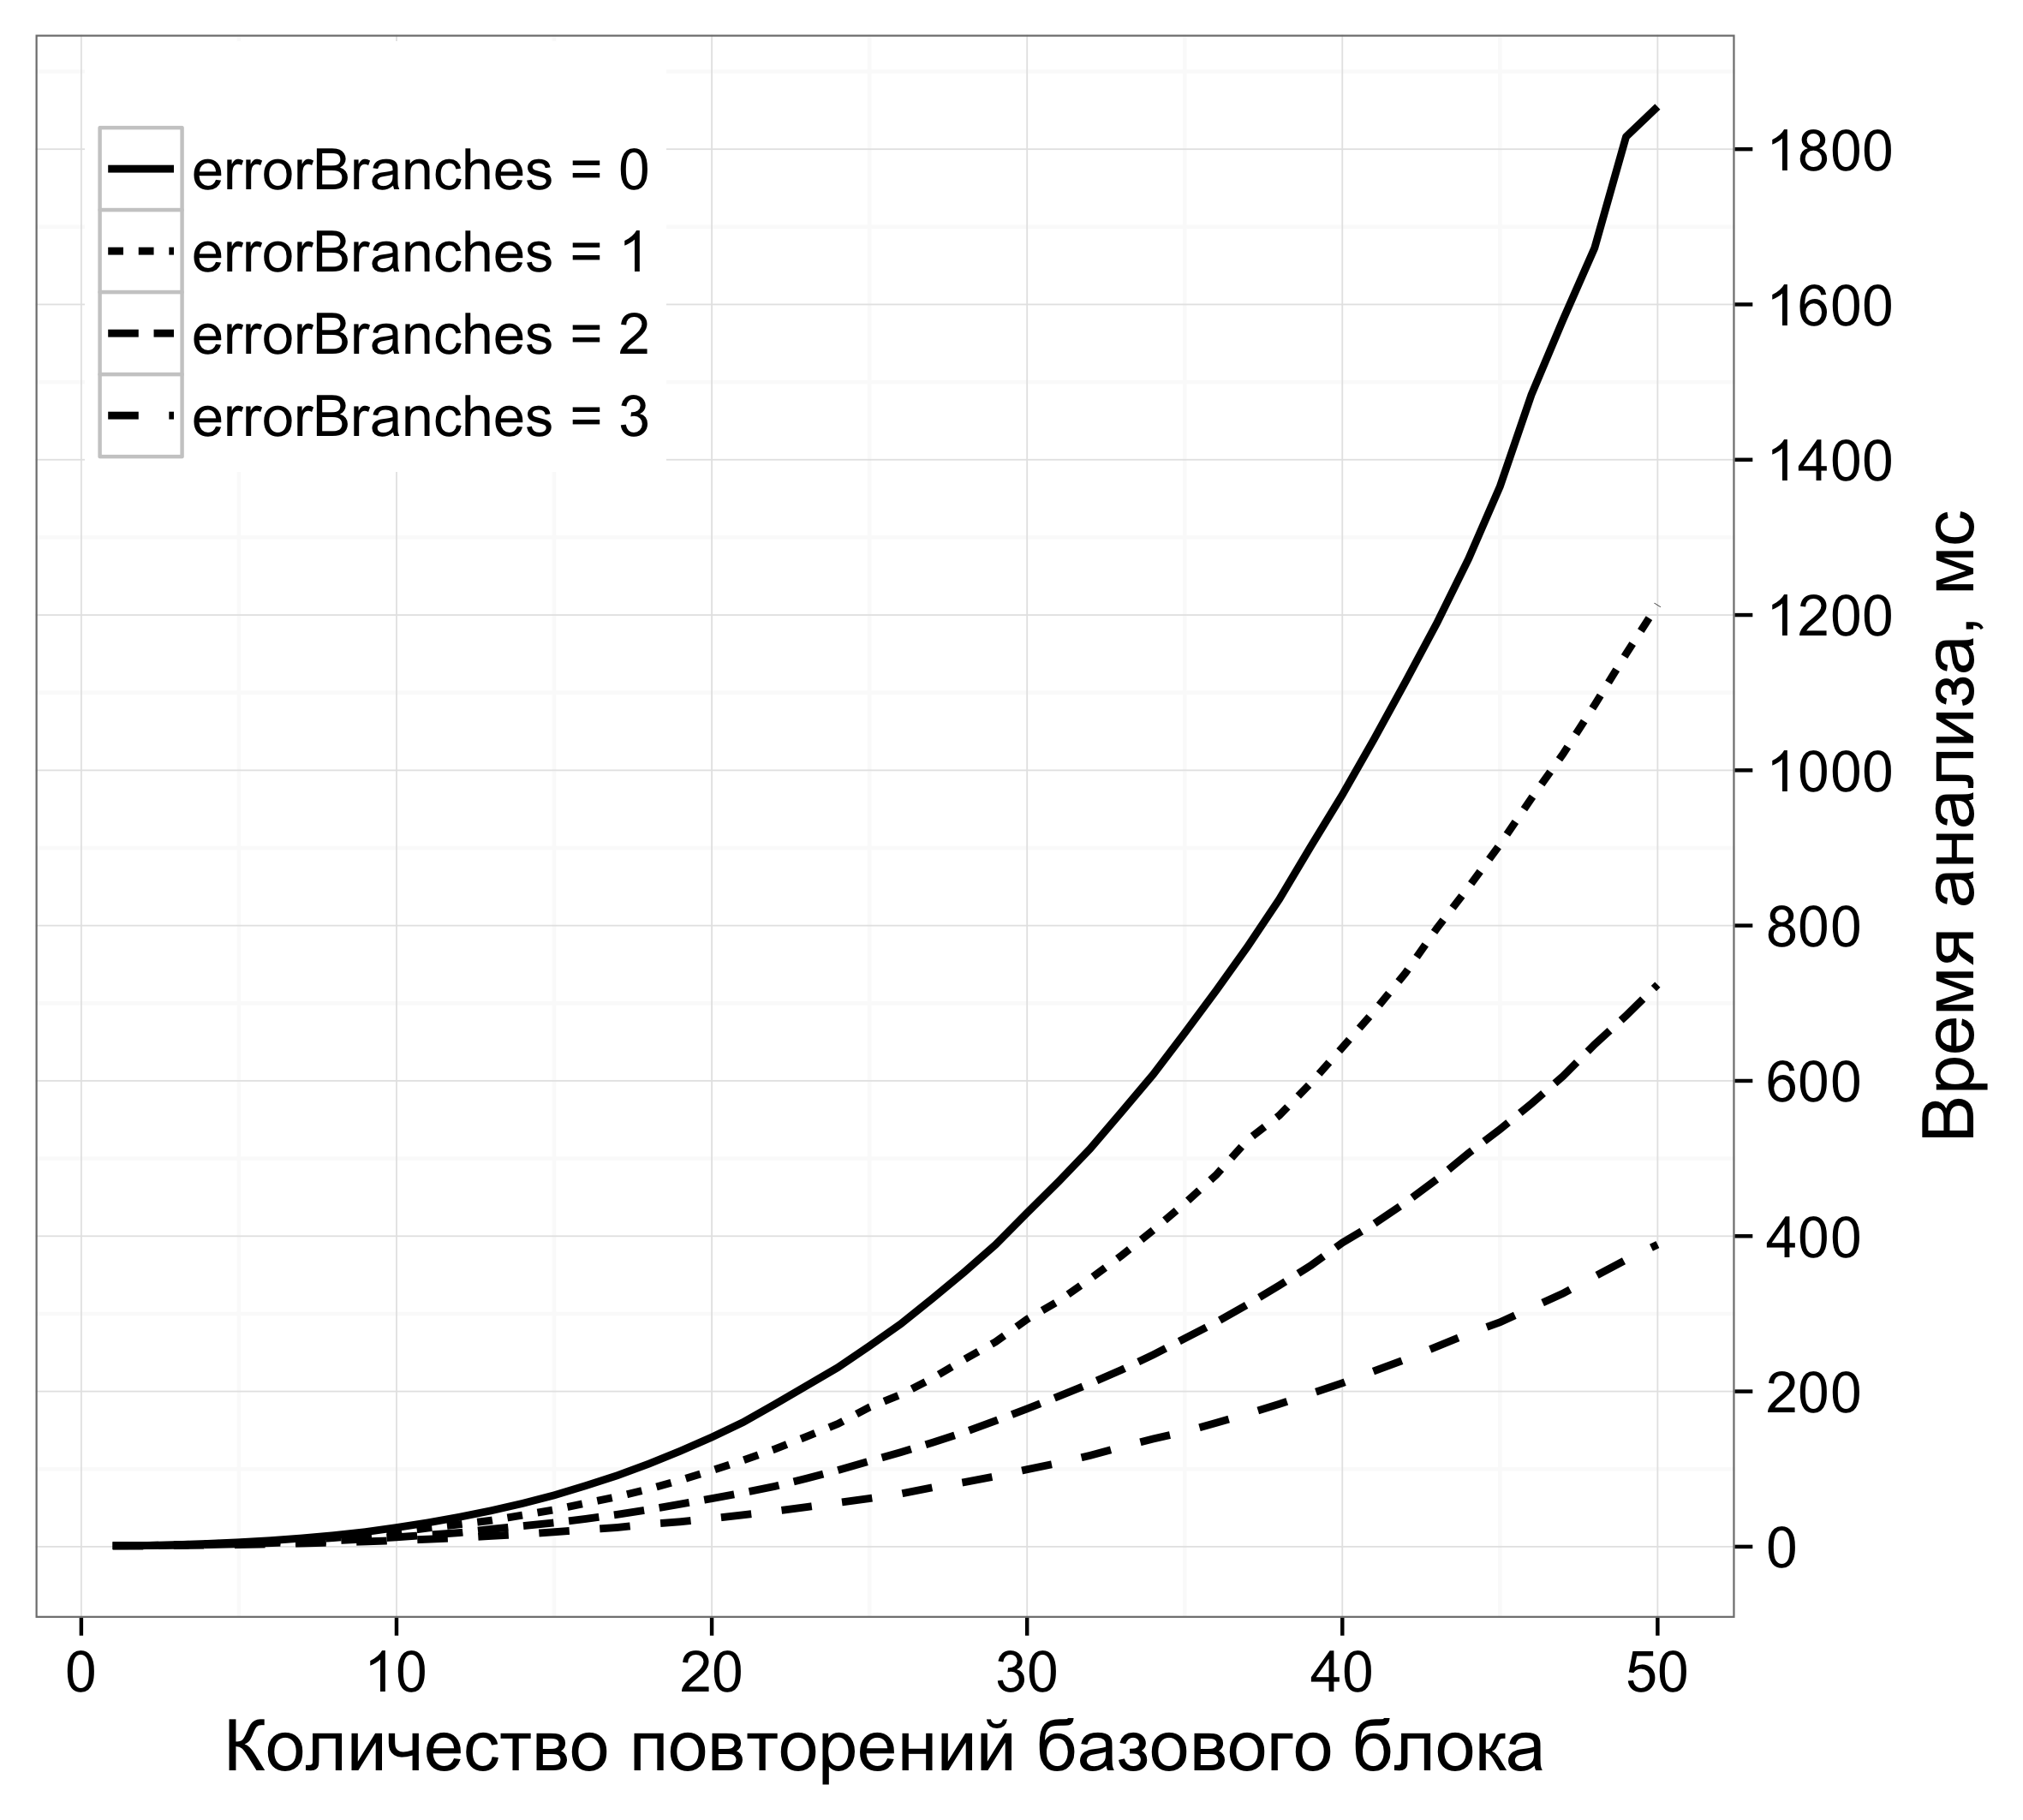
\includegraphics[width=11cm]{pictures/error_branches4_black.png}
 \caption{Зависимость времени работы модифицированного алгоритма от размера входного графа и количества ошибочных ребер при $height=6$}
 \label{withErrors}
\end{figure}
\clearpage